\section{Filtering in the frequency domain \buch{p.199}}
\subsection{Countinous Fourier Transform \buch{p.205}}
\subsection{Sampling \buch{p.211}}
Multiplication of the function with an impulse train
\begin{equation}
\tilde{f}(t) = f(t) s_{\Delta T}(t) = \sum_{n=-\infty}^{\infty}f(t)\sigma (t-n \Delta T)
\end{equation}
The fourier transform of it
\begin{equation}
\tilde{F}(\mu) = F(\mu) \star S(\mu) = \frac{1}{\Delta T} \sum_{n=-\infty}^{\infty}F\left(\mu - \frac{n}{\Delta T}\right)
\end{equation}

\subsection{The discrete Fourier transform of one variable \buch{p.220}}
The Fourier transform of sampled data is continuous and infinitely periodic with period $1/\Delta T$
\begin{equation}
\tilde{F}(\mu)= \sum_{n=-\infty}^{\infty} f_n \cdot e^{-j 2 \pi  \mu n \Delta T}
\end{equation}

We are only interested in one period.
So we obtain $M$ equally spaced samples of $\tilde{F}(\mu)$ over the period $\mu = 0$ to $\mu = 1/\Delta T$
\begin{equation}
\mu = \frac{m}{M \Delta T}
\end{equation}

This results in

\begin{equation}
F_m = \sum_{n=0}^{M-1} f_n \cdot e^{-j 2 \pi m n / M} \quad m = 0,1,2,\dots,M-1
\end{equation}
 
The \emph{inverse discrete Fourier transform} is used to recover the sample set ${f_n}$
\begin{equation}
f_n = \frac{1}{M} \sum_{m=0}^{M-1}F_m e^{j 2 \pi m n / M} \quad n = 0,1,2,\dots,M-1
\end{equation}

\begin{itemize}
\item The discrete Fourier transform is an invertible, linear transformation
\item The DFT pair is applicable to \emph{any} finite set of uniformly discrete samples
\item DFT and IDFT are periodic with period M
\end{itemize}
 
\subsubsection{Sampling and Frequency Intervals \buch{p.223}}
If $f(x)$ consists of $M$ samples, taken $\Delta T$ units apart, the duration $T$ of the record is
\begin{equation}
	T = M \Delta T
\end{equation}
The corresponding spacing in the discrete frequency domain $\Delta u$ is
\begin{equation}
	\Delta u = \frac{1}{M \Delta T} = \frac{1}{T}
\end{equation}
The frequency range spanned by the $M$ components of the DFT is
\begin{equation}
	\Omega = M \Delta u = \frac{1}{\Delta T}
\end{equation} 

\subsection{2D Countinous FT \buch{p.205}} 
\subsection{The 2D Impulse \buch{p.225}}
The discrete 2D impulse is defined as
\begin{equation}
\delta(x,y) = 
\begin{cases} 1 & \text{if $x=y=0$,}
\\
0 &\text{otherwise}
\end{cases}
\end{equation}

with the sifting property
\begin{equation}
\sum_{x=-\infty}^{\infty}\sum_{y=-\infty}^{\infty}f(x,y) \delta(x,y) = f(0,0)
\end{equation}

\subsection{2D Sampling Theorem}
A continuous, band-limited function $f(t,z)$ can be recovered with no error if the sampling intervals are\\
 \begin{minipage}{0.4\textwidth}
   \[
   \Delta T < \dfrac{1}{2 u_{max}}
   \]
 \end{minipage} 
and
  \begin{minipage}{0.4\textwidth}
    \[
    \Delta Z < \dfrac{1}{2 v_{max}}
    \]
  \end{minipage} 
  
  

\subsection{2D DFT and IDFT \buch{p.235}}

\subsubsection{2D DFT}
\begin{equation}
    F(u,v) = \sum_{x=0}^{M-1}\sum_{y=0}^{N-1}f(x,y)\cdot e^{-j2\pi \left(\frac{ux}{M}+ \frac{vy}{N}\right)}
\end{equation}
\begin{center}
  with $u$ and $v$ in the ranges $u = 0,1,2,\ldots,M-1$ and $v = 0,1,2,\ldots,N-1$
\end{center}
\subsubsection{2D IDFT}
\begin{equation}
    f(x,y) = \frac{1}{MN} \sum_{u=0}^{M-1}\sum_{v=0}^{N-1}F(u,v)\cdot e^{j2\pi \left(\frac{ux}{M}+ \frac{vy}{N}\right)}
\end{equation}
\begin{center}
  with $x$ and $y$ in the ranges $x = 0,1,2,\ldots,M-1$ and $y = 0,1,2,\ldots,N-1$
\end{center}

\subsubsection{Properties}
\begin{itemize}
\item Separation between samples in the frequency domain are inversely proportional to the spacing between spatial samples and the number of samples
$\Delta u = \frac{1}{M \Delta T} \quad \Delta v = \frac{1}{N \Delta Z}$
\item Infinitely periodic
\item Symmetry properties \buch{p.242}, see Table \ref{tab:Symmetry_2D_DFT} (Appendix)
\item Summary of properties \buch{p.253}, see Table \ref{tab:Properties_2D_DFT} and \ref{tab:DFT_Pairs} (Appendix)
\end{itemize}

\subsubsection{Periodicity \buch{237}}
  Visualization is simplified if we shift the data so that F(0,0) at (M/2,N/2) with
    \begin{equation}
      f(x,y)(-1)^{x+y} \Leftrightarrow F(u-M/2, v-N/2)
    \end{equation}
    
\subsubsection{"DC"}
  \begin{equation}
    |F(0,0)| = MN|\bar{f}(x,y)|
  \end{equation}

\subsubsection{2-D Convolution \buch{p.249}}
The 2-D Convolution Theorem is given by:
\begin{align}
	f(x,y) \bigstar h(x,y) \Leftrightarrow F(u,v)H(u,v)
\end{align}

It is necessairy to zero-pad the images $f(x,y)$ of size $A \times B$ and $h(x,y)$ of size $C \times D$ as follows:

\begin{equation}
	f_p(x,y) = 
		\begin{cases} 
			f(x,y) & 0 \leq x \leq A-1 \text{  and  } 0 \leq y \leq B-1 \\
			0 & A \leq x \leq P \text{  or  } B \leq y \leq Q
		\end{cases}
\end{equation}
\begin{equation}
	h_p(x,y) = 
		\begin{cases}
			h(x,y) & 0 \leq x \leq C-1 \text{  and  } 0 \leq y \leq D-1 \\
			0 & C \leq x \leq P \text{  or  } D \leq y \leq Q
		\end{cases}
\end{equation}
with
\begin{align}
	P &\geq A+C-1 \\
	Q &\geq B+D-1
	\label{equ:2D_Conv_Padding}
\end{align}
resulting in padded images of size $P \times Q$

\subsection{Basics of Filtering in the Frequency Domains}
  Generally, filtering in the frequency domain is obtained by
  \begin{equation}
  g(x,y) = \Im^{-1} \left[ H(u,v) F(u,v) \right]
  \end{equation}
  if filter $H(u,v)$ is real \& symmetric
  \begin{equation}
  g(x,y) = \Im^{-1} \left[ H(u,v) \cdot R(u,v) + j H(u,v) \cdot I(u,v)\right]
  \end{equation}  
  $\Rightarrow$ Filter that affect real and imaginary parts equally have no effect on the phase $\rightarrow$ \textbf{zero-phase-shift} filters 

\subsubsection{Summary of Steps for Filtering in the Frequency Domain \buch{p.263}}
  
\begin{enumerate}
	\item Given an input image $f(x,y)$ of size $M \times N$, obtain the padding parameters $P$ and $Q$ from Eq. \ref{equ:2D_Conv_Padding}. Typically, we select $P=2M$ and $Q=2N$.
	\item Form a padded image, $f_p(x,y)$, of size $P \times Q$ by appending the necessary number of zeros to $f(x,y)$.
	\item Multiply $f_p(x,y)$ by $(-1)^{x+y}$ to center its transform.
	\item Compute the DFT, $F(u,v)$, of the image from step 3.
	\item Generate a real, symmetric filter function, $H(u,v)$, of size $P \times Q$ with center at coordinates $(P/2,Q/2)$. Form the product $G(u,v) = H(u,v) F(u,v)$ using array multiplication.
	\item Obtain the processed image, $g_p(x,y) = \left\lbrace \text{real} \left[ \Im^{-1} \left[ G(u,v) \right] \right] \right\rbrace (-1)^{x+y}$, where the real part is selected in order to ignore parasitic complex components resulting from computational inaccuracies, and the subscript $p$ indicates that we are dealing with padded arrays.
	\item Obtain the final processed result, $g(x,y)$, by extracting the $M \times N$ region from the top, left quadrant of $g_p(x,y)$.
\end{enumerate}

\subsection{Image smoothing using frequency domain filters \buch{p.269}}
\subsubsection{Ideal Lowpass Filters}
\begin{equation}
	H(u,v)  = 
		\begin{cases}
			1 & \text{  if } D(u,v) \leq D_0 \\
			0 & \text{  if } D(u,v) > D_0 \\ 
		\end{cases}
\end{equation}
where $D_0$ is a positive constant and $D(u,v)$ is the distance between a point $(u,v)$ in the frequency domain and the center of the frequency rectangle; that is,
\begin{equation}
	D(u,v) = \left[ (u-P/2)^2 + (v-Q/2)^2 \right]^{1/2}
	\label{equ:Freq_Filter_D_uv}
\end{equation}
ILPFs have a \textbf{huge ringing problem} and are not frequently used.

\subsubsection{Butterworth Lowpass Filters}
The transfer function of a Butterworth lowpass filter (BLPF) of order $n$, and with cutoff frequency at a distance $D_0$ from the origin, is defined as
\begin{equation}
	H(u,v) = \frac{1}{1 + \left[ D(u,v) / D_0 \right]^{2n}}
\end{equation}
The BLPF of order 1 has no ringing, but ringing can become significant in filters of higher order. Usually only BLPFs with $n \leq 4$ are used.

\subsubsection{Gaussian Lowpass Filters}
A Gaussian lowpass filter (GLPF) of two dimensions is given by
\begin{equation}
	H(u,v) = e^{-D^2(u,v)/2D_0^2}
\end{equation}
where $D_0$ is the cutoff frequency. When $D(u,v)=D_0$, the GLPF is down to $0.607$ of its maximum value. The GLPF will have \textbf{no ringing}.

\subsection{Image sharpening using frequency domain filters \buch{p.280}}
A highpass filter is obtained from a given lowpass filter by
\begin{equation}
	H_{HP}(u,v) = 1 - H_{LP}(u,v)
\end{equation}

\subsubsection{Ideal Highpass Filters}
A ideal highpass filter (IHPF) is defined as
\begin{equation}
	H(u,v) = 
		\begin{cases}
			0 & \text{  if } D(u,v) \leq D_0 \\
			1 & \text{  if } D(u,v) > D_0
		\end{cases}
\end{equation}
where $D_0$ is the cutoff frequency and $D(u,v)$ is given by Eq. \ref{equ:Freq_Filter_D_uv}. Like the ILPF, the IHPF creates a large ringing.

\subsubsection{Butterworth Highpass Filters}
A 2-D Butterworth highpass filter (HBPF) of order $n$ and cutoff frequency $D_0$ is defined as 
\begin{equation}
	H(u,v) = \frac{1}{1 + \left[ D_0 / D(u,v) \right]^{2n}}
\end{equation}

\subsubsection{Gaussian Highpass Filters}
The transfer function of the Gaussian highpass filter (GHPF) with cutoff frequency at $D_0$ is given by
\begin{equation}
	H(u,v) = 1 - e^{-D^2(u,v)/2D_0^2}
\end{equation}

\subsubsection{The Laplacian in the Frequency Domain \buch{p.286}}
The Laplacian can be implemented in the frequency domain using the filter
\begin{equation}
	H(u,v) = -4 \pi^2 D^2(u,v)
	\label{equ:Laplacian_Freq_Domain}
\end{equation}
The Laplacian image is obtained as
\begin{equation}
	\nabla^2 f(x,y) = \Im^{-1} \left\lbrace H(u,v)F(u,v) \right\rbrace 
\end{equation}

The enhanced image $g(x,y) = f(x,y) + c \nabla^2f(x,y)$ with $c=-1$ can be achieved by
\begin{equation}
	g(x,y) = \Im^{-1} \left\lbrace \left[ 1 + 4 \pi^2 D^2(u,v) \right] F(u,v) \right\rbrace 
\end{equation}

Usually, $f(x,y)$ is normalized to the range $\left[0,1\right]$ and $\nabla^2 f(x,y)$ is divided by its maximum value, which brings it to the approximate range $\left[-1,1\right]$.

\subsubsection{Unsharp Masking, Highboost Filtering, and High-Frequency-Emphasis Filtering \buch{p.288}}
A high-frequency-emphasis filter is achieved by
\begin{equation}
	g(x,y) = \Im^{-1} \left\lbrace \left[ k_1 + k_2 \cdot H_{HP}(u,v) \right] F(u,v) \right\rbrace 
\end{equation}
where $k_1 \geq 0$ gives control of the offset from the origin and $k_2 \geq 0$ controlls the contribution of high frequencies.

\subsubsection{Homomorphic Filtering \buch{p.290}}
\begin{minipage}{9cm}
	Homomorphic filtering is used to separate illumination and reflectance components. This is achieved by using the natural logarithm $\ln$ before applying the DFT.
\end{minipage}
\begin{minipage}{9cm}
	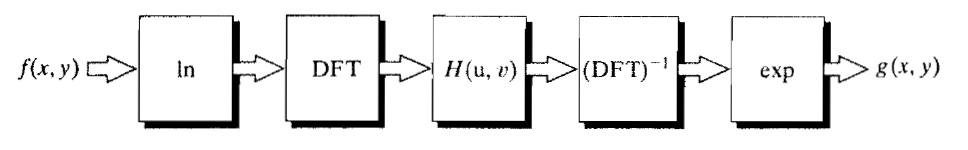
\includegraphics[width=9cm]{images/Homomorphic_Filtering.png}
	%TODO: Bild vertikzisieren
\end{minipage} \\

A modified version of a Gaussian highpass,
\begin{equation}
	H(u,v) = (\gamma_H - \gamma_L) \left[ 1 - e^{-c \left[ D^2(u,v) / D_0^2 \right]} \right] + \gamma_L
\end{equation}
allows to attenuate the low frequencies (illumination) with $\gamma_L < 1$ and amplify the high frequencies (reflectance) with $\gamma_H > 1$.


\subsection{Selective Filtering \buch{p.294}}

\subsubsection{Bandreject and Bandpass Filters} \label{subsubsec:FilteringFrequency_BandrejectFilters}
Bandreject filters are given by the following equations,

\begin{table}[htbp]
	\centering
	\begin{tabular}{|ccc|}
		\hline
		\textbf{Ideal} & \textbf{Butterworth} & \textbf{Gaussian} \\ \hline
		$H(u,v) = 
			\begin{cases}
				0 & \text{  if } D_0-\frac{W}{2} \leq D \leq D_0 + \frac{W}{2} \\
				1 & \text{  otherwise}
			\end{cases} $
		& $H(u,v) = \frac{1}{1 + \left[ \frac{DW}{D^2 - D_0^2} \right]^{2n}}$
		& $H(u,v) = 1-e^{-\left[\frac{D^2-D_0^2}{DW}\right]^2}$ \\
		\hline
	\end{tabular}
\end{table}

where $D_0$ is the radial center of the band, $W$ is the width of the band, and $D(u,v)$ is given by Eq. \ref{equ:Freq_Filter_D_uv}. \\

A bandpass filter is obtained by
\begin{equation}
	H_{BP}(u,v) = 1 - H_{BR}(u,v)
\end{equation}

\subsubsection{Notch Filters}  \label{subsubsec:FilteringFrequency_NotchFilters}
A notch filter rejects (or passes) frequencies in a predefined neighborhood about the center of the frequency rectangle. Notch reject filters are constructed as products of highpass filters whose centers have been translated to the centers of the notches. The general form is
\begin{equation}
	H_{NR}(u,v) = \prod_{k=1}^{Q} H_k(u,v) H_{-k}(u,v)
\end{equation}
where $H_k(u,v$ and $H_{-k}(u,v)$ are highpass filters whose centers are at $(u_k,v_k)$ and $(-u_k,-v_k)$. \\

A notch pass filter is obtained from a notch reject filter by
\begin{equation}
	H_{NP}(u,v) = 1 - H_{NR}(u,v)
\end{equation}

\subsection{Implementation \buch{p.298}}